
% Springer Nature article template - clean starting point
% Based on the supplied sn-article.tex template.

\documentclass[pdflatex,sn-mathphys-num]{sn-jnl}

% Standard packages from the Springer template
\usepackage{graphicx}
\usepackage{multirow}
\usepackage{amsmath,amssymb,amsfonts}
\usepackage{amsthm}
\usepackage{mathrsfs}
\usepackage[title]{appendix}
\usepackage{xcolor}
\usepackage{textcomp}
\usepackage{manyfoot}
\usepackage{booktabs}
\usepackage{algorithm}
\usepackage{algorithmicx}
\usepackage{algpseudocode}
\usepackage{listings}
\usepackage{booktabs}
\usepackage{placeins}

% Theorem environments from the Springer template
\theoremstyle{thmstyleone}
\newtheorem{theorem}{Theorem}
\newtheorem{proposition}[theorem]{Proposition}

\theoremstyle{thmstyletwo}
\newtheorem{example}{Example}
\newtheorem{remark}{Remark}

\theoremstyle{thmstylethree}
\newtheorem{definition}{Definition}

\raggedbottom

\begin{document}

% ------------------------------------------------------------
% Title and authors
% ------------------------------------------------------------

\title[Short Title]{Your Research Paper Title}

\author*[1]{\fnm{First} \sur{Author}}\email{your.email@example.com}

\affil*[1]{\orgdiv{Department},
\orgname{Institution},
\orgaddress{\city{City}, \postcode{000000}, \state{State}, \country{Country}}}

% Add more authors/affiliations using the Springer commands above as needed.

% ------------------------------------------------------------
% Abstract and keywords
% ------------------------------------------------------------

\abstract{Write your abstract here. The abstract should briefly describe the research problem, methodology, main results, and conclusions.}

\keywords{keyword one, keyword two, keyword three, keyword four}

\maketitle

% ------------------------------------------------------------
% Main paper
% ------------------------------------------------------------

\section{Introduction}\label{sec:introduction}
Write your introduction here. Explain the background, research problem, motivation, objectives, and contributions of the work.

\section{Related Work}\label{sec:related-work}

Review the relevant literature and explain how your work relates to existing research.

\section{Methodology}\label{sec:methodology}

\subsection{Dataset Description}\label{subsec:dataset}

This study uses Automatic Identification System (AIS) data
obtained from Global Fishing Watch (GFW) to examine the
spatiotemporal distribution of fishing activity. The dataset
consists of daily observations associated with individual
vessels and geographical grid cells, covering the period
from February 2012 to December 2024.

Each observation contains six primary variables, as
illustrated in Table~\ref{tab:dataset-sample}.

\begin{table}[t]
\caption{Representative observations from the AIS dataset.}
\label{tab:dataset-sample}
\begin{tabular}{llllrr}
\toprule
Date & Latitude & Longitude & MMSI & Hours & Fishing hours \\
\midrule
02-01-2023 & -73.0 & 179.6  & 440203000 & 2.2997  & 0.8833 \\
02-01-2023 & -72.9 & 178.0  & 512006000 & 2.8822  & 1.5816 \\
02-01-2023 & -72.7 & -179.3 & 272364000 & 0.6338  & 0.0000 \\
31-03-2023 & -63.0 & -57.3  & 272208000 & 1.3694  & 0.9111 \\
31-03-2023 & -63.0 & -57.5  & 272208000 & 6.7194  & 5.6647 \\
31-03-2023 & -62.7 & -55.0  & 725001619 & 16.4736 & 15.6769 \\
\botrule
\end{tabular}
\end{table}

The variables represent the following information:
\textit{date} indicates the observation date;
\textit{cell\_ll\_lat} and \textit{cell\_ll\_lon}
represent the latitude and longitude of the lower-left
corner of the corresponding spatial grid cell;
\textit{mmsi} identifies the vessel using its Maritime
Mobile Service Identity; \textit{hours} represents
the total observed activity hours; and
\textit{fishing\_hours} represents the estimated
hours of fishing activity.

Following data integration and cleaning, the dataset
contains 730,488 observations, representing 1,930
unique vessels and 23,846 distinct spatial grid cells.
The geographical coverage extends from
$-29.2^\circ$ to $40.0^\circ$ latitude and
$32.0^\circ$ to $161.9^\circ$ longitude.

The source observations are already filtered to
include fishing-active records. Therefore,
\textit{fishing\_hours} is used as the primary
measure of fishing effort in this study.


\subsection{Data Preprocessing}\label{subsec:preprocessing}

The original dataset was distributed as multiple daily
CSV files organized by month and year. Before conducting the
spatiotemporal analysis, these files were integrated into
a standardized dataset through a preprocessing pipeline.
The primary objective was to ensure consistent data
representation, validate the temporal and spatial
attributes, and prepare the observations for subsequent
aggregation.

\subsubsection{Daily Observation Integration}

The original dataset consisted of multiple CSV files
containing daily AIS observations. Each record represents
the observed activity of a vessel within a specific
geographical grid cell on a particular date.

To facilitate the analysis, the individual files were
combined into a single dataset. During integration,
two different CSV structures were encountered: files
containing column headers and files without headers.
For files without headers, the expected column names
were explicitly assigned to ensure a consistent
data structure.

Following this standardization, all observations
were concatenated into a unified dataset, providing
a consistent foundation for subsequent data
cleaning and spatiotemporal analysis.

\subsubsection{Data Cleaning and Validation}

The date variable was converted into a standardized
datetime representation using mixed-format date parsing.
The geographical coordinates, vessel identification
numbers, and activity-hour variables were converted
into numeric data types to ensure consistency during
subsequent computations.

Records containing missing or invalid values in the
required analytical columns were excluded through
complete-case filtering. The extracted year, month, and
day components were also derived from the standardized
date variable.

Several validation procedures were performed to assess
the quality of the integrated dataset. These included:

\begin{itemize}
    \item Verification of the correspondence between
    the dates and the year and month indicated by
    their respective source files.

    \item Identification of missing values and
    duplicate observations.

    \item Examination of negative values in the
    total activity hours and fishing hours variables.

    \item Validation of geographical coordinates
    against the permissible latitude and longitude
    ranges.

    \item Examination of coordinate intervals to
    verify consistency with the native spatial grid.
\end{itemize}

The validation process identified no missing values,
negative activity-hour values, or geographically
invalid coordinates in the resulting dataset. A total
of 78 duplicate rows were identified during the quality
checks.

\subsubsection{Spatial and Temporal Representation}

Each observation was retained at its original
date--spatial cell--vessel level. The geographical
coordinates were preserved using the native grid
representation provided by Global Fishing Watch.
No additional spatial re-gridding was performed.

The availability of observations varied across the
study period. Although the dataset contains monthly
files spanning 2012--2024, some months are unavailable
in the earlier years. Therefore, missing months were
not interpreted as periods with zero fishing activity
and were not artificially populated with zero values.

For the temporal trend analysis, the period
2015--2024 was selected because it provides
substantially more complete temporal coverage than
the earlier years.

Following preprocessing, the standardized dataset
was stored in Parquet and CSV formats for use in
subsequent analytical stages.


\subsection{Fishing Effort Estimation}\label{subsec:fishing-effort}

Fishing effort was quantified using the estimated
fishing hours associated with each AIS observation.
Since the source dataset contains fishing-active
observations, the sum of fishing hours provides the
primary measure of observed fishing effort used
throughout this study.

The estimation procedure consists of aggregating
individual observations across geographical cells
and temporal intervals to characterize the distribution
and evolution of fishing activity.


\subsubsection{Monthly Spatial Aggregation}

Let $i$ represent an individual AIS observation,
$c$ a geographical grid cell, $y$ a calendar year,
and $m$ a calendar month.

The monthly fishing effort for a geographical cell
is calculated by summing the fishing hours of all
observations associated with that cell during the
corresponding month.

The monthly fishing effort is therefore expressed as:

\begin{equation}
E_{c,y,m} =
\sum_{i \in \mathcal{O}_{c,y,m}}
f_i
\label{eq:monthly-effort}
\end{equation}

where:

\begin{itemize}
    \item $E_{c,y,m}$ represents the total fishing effort
    in cell $c$ during month $m$ of year $y$.

    \item $\mathcal{O}_{c,y,m}$ denotes the set of
    observations associated with the corresponding
    spatial cell and month.

    \item $f_i$ represents the fishing hours recorded
    for observation $i$.
\end{itemize}

In addition to fishing effort, other activity indicators
were calculated for each cell-month combination.
These include total observed activity hours, the
number of distinct active vessels, and the number
of distinct observed activity dates.

The total observed activity hours are calculated as:

\begin{equation}
H_{c,y,m} =
\sum_{i \in \mathcal{O}_{c,y,m}} h_i
\label{eq:total-hours}
\end{equation}

where $h_i$ represents the total observed activity
hours associated with observation $i$.

The number of active vessels and active days are
calculated using the number of unique vessel
identifiers and observation dates, respectively.

A supplementary fishing ratio is also derived as:

\begin{equation}
R_{c,y,m} =
\frac{E_{c,y,m}}{H_{c,y,m}}
\label{eq:fishing-ratio}
\end{equation}

This ratio represents the proportion of total
observed activity hours attributed to fishing.
However, it is treated as a supplementary
indicator rather than the primary measure
of fishing effort.


\subsubsection{Annual Fishing Effort}

To investigate longer-term variations in fishing
activity, monthly observations were further
aggregated into annual measurements for each
geographical cell.

The annual fishing effort is calculated by summing
the monthly fishing hours available within a given
cell and year:

\begin{equation}
E_{c,y} =
\sum_{m \in \mathcal{M}_{c,y}}
E_{c,y,m}
\label{eq:annual-effort}
\end{equation}

where $\mathcal{M}_{c,y}$ denotes the set of
months for which observations are available
in cell $c$ during year $y$.

The number of months with available observations
is recorded for each cell-year combination.
Annual cell records containing observations from
fewer than three months are excluded from the
subsequent trend analysis.

Additionally, the number of unique active vessels
is calculated independently at the annual level.
This avoids double-counting vessels that appear
in multiple months within the same geographical
cell and year.


\subsubsection{Normalization of Fishing Effort}

Annual fishing effort can be influenced by
differences in the number of months for which
observations are available. Comparing annual
totals without considering this variation may
introduce bias when examining temporal changes.

To address this issue, mean monthly fishing
effort is calculated for each cell-year
combination:

\begin{equation}
\overline{E}_{c,y} =
\frac{E_{c,y}}{M_{c,y}}
\label{eq:mean-monthly-effort}
\end{equation}

where $M_{c,y}$ represents the number of months
with available observations in cell $c$ during
year $y$.

This measure provides a coverage-normalized
representation of fishing effort by expressing
the annual accumulated fishing hours as an
average over the observed months.

The mean monthly fishing effort is subsequently
used as the primary variable for estimating
cell-level temporal trends, while the raw annual
fishing effort is retained for descriptive
comparisons.

% Example subsection:
% \subsection{Data Collection}\label{subsec:data-collection}
% Write the subsection content here.



\section{Results}\label{sec:results}

% ------------------------------------------------------------
% 4.1 Temporal Coverage and Overall Fishing Effort
% ------------------------------------------------------------

\subsection{Temporal Coverage and Overall Fishing Effort}
\label{subsec:overall-results}

The temporal analysis was conducted over the period
2015--2024, which provides more consistent data
availability than the earlier years. Although the
dataset contains observations from 2012 onwards,
the availability of monthly observations varies
considerably during the initial years.

Across the selected study period, the total recorded
fishing hours increased from 7,834.25 hours in 2015
to 846,165.09 hours in 2024. However, this increase
was accompanied by a substantial expansion in the
number of observed spatial cells, from 578 in 2015
to 15,914 in 2024.

The highest recorded annual fishing effort was
observed in 2023, with 991,262.66 hours. A reduction
to 846,165.09 hours was observed in 2024. These
variations should be interpreted in conjunction
with the changing spatial coverage of the dataset,
rather than as direct evidence of changes in
overall fishing intensity.

\begin{table}[!htbp]
\centering
\caption{Annual observed fishing effort and spatial
coverage during 2015--2024.}
\label{tab:annual-effort}
\small
\begin{tabular}{lrr}
\toprule
Year & Fishing hours & Observed cells \\
\midrule
2015 & 7,834.25 & 578 \\
2016 & 7,963.53 & 1,155 \\
2017 & 21,215.11 & 895 \\
2018 & 65,335.07 & 1,811 \\
2019 & 81,839.88 & 2,411 \\
2020 & 41,358.30 & 1,494 \\
2021 & 220,120.44 & 4,887 \\
2022 & 771,036.06 & 11,332 \\
2023 & 991,262.66 & 15,134 \\
2024 & 846,165.09 & 15,914 \\
\bottomrule
\end{tabular}
\end{table}

\FloatBarrier


% ------------------------------------------------------------
% 4.2 Spatial Distribution of Fishing Effort
% ------------------------------------------------------------

\subsection{Spatial Distribution of Fishing Effort}
\label{subsec:spatial-results}

The spatial aggregation of fishing hours revealed
considerable variation in the distribution of
fishing activity across geographical grid cells.
Over the complete study period, certain spatial
cells accumulated substantially higher fishing
effort than others.

The cell located at $12.8^\circ$ N and
$74.6^\circ$ E recorded the highest accumulated
fishing effort, with 22,251.96 fishing hours and
643 distinct vessels. Other high-effort cells
were also identified in the surrounding
geographical region.

Table~\ref{tab:top-effort-cells} presents the
five spatial cells with the highest accumulated
fishing effort across the available study period.

\begin{table}[!htbp]
\centering
\caption{Five spatial cells with the highest
accumulated fishing effort.}
\label{tab:top-effort-cells}
\small
\begin{tabular}{rrrr}
\toprule
Latitude & Longitude & Fishing hours & Vessels \\
\midrule
12.8 & 74.6 & 22,251.96 & 643 \\
12.7 & 74.6 & 19,798.00 & 605 \\
12.6 & 74.7 & 17,814.98 & 538 \\
12.7 & 74.7 & 16,075.32 & 561 \\
12.9 & 74.5 & 15,299.72 & 604 \\
\bottomrule
\end{tabular}
\end{table}

\FloatBarrier


% ------------------------------------------------------------
% 4.3 Spatially Resolved Temporal Trends
% ------------------------------------------------------------

\subsection{Spatially Resolved Temporal Trends}
\label{subsec:trend-results}

Temporal trends were estimated independently
for each geographical grid cell using mean
monthly fishing hours as the primary analytical
variable. A minimum of five annual observations
was required for a cell to be considered eligible
for trend estimation.

A total of 8,697 spatial cells were examined,
of which 557 satisfied the minimum temporal
observation requirement. The remaining 8,140
cells were classified as having insufficient
data for trend estimation.


% ------------------------------------------------------------
% 4.3.1 Classification of Fishing-Effort Trends
% ------------------------------------------------------------

\subsubsection{Classification of Fishing-Effort Trends}

Based on the estimated linear regression slopes
and a statistical significance threshold of
$p < 0.05$, the eligible spatial cells were
classified into increasing, declining, and
stable or statistically non-significant trends.

Among the 557 eligible cells, 511 (91.74\%)
were classified as stable or statistically
non-significant. A total of 39 cells (7.00\%)
exhibited statistically significant increasing
trends, whereas 7 cells (1.26\%) exhibited
statistically significant declining trends.

The overall distribution of trend classifications
is presented in Table~\ref{tab:trend-classification}.

\begin{table}[!htbp]
\centering
\caption{Distribution of spatial cells according
to estimated fishing-effort trends.}
\label{tab:trend-classification}
\small
\begin{tabular}{lrr}
\toprule
Trend category & Number of cells & Percentage of all cells (\%) \\
\midrule
Insufficient data & 8,140 & 93.60 \\
Stable / not significant & 511 & 5.88 \\
Increasing & 39 & 0.45 \\
Declining & 7 & 0.08 \\
\midrule
Total & 8,697 & 100.00 \\
\bottomrule
\end{tabular}
\end{table}

\FloatBarrier

Considering only the 557 eligible cells,
the declining and increasing categories
represent 1.26\% and 7.00\%, respectively.
The predominance of statistically non-significant
cells indicates that clear linear trends were
not detected in most of the spatial cells
with sufficient temporal observations.


% ------------------------------------------------------------
% 4.3.2 Regions Exhibiting Declining Fishing Effort
% ------------------------------------------------------------

\subsubsection{Regions Exhibiting Declining Fishing Effort}

Seven spatial cells exhibited statistically
significant declining fishing-effort trends.
These cells were primarily located between
$17.0^\circ$--$18.6^\circ$ N latitude and
$72.0^\circ$--$72.8^\circ$ E longitude.

The strongest negative trend was identified
at the cell located at $18.5^\circ$ N and
$72.0^\circ$ E, with an estimated slope of
$-10.8746$ mean monthly fishing hours per year.
The corresponding coefficient of determination
was $R^2 = 0.8380$, with a regression
$p$-value of 0.0291.

The estimated trends for all seven declining
cells are presented in Table~\ref{tab:declining-cells}.

\begin{table}[!htbp]
\centering
\caption{Spatial cells exhibiting statistically
significant declining fishing-effort trends.}
\label{tab:declining-cells}
\small
\begin{tabular}{rrrrrr}
\toprule
Latitude & Longitude & Years & Slope & $R^2$ & $p$-value \\
\midrule
18.5 & 72.0 & 5 & -10.8746 & 0.8380 & 0.0291 \\
17.0 & 72.8 & 8 & -8.7219 & 0.5152 & 0.0450 \\
18.5 & 72.4 & 5 & -6.5667 & 0.9263 & 0.0087 \\
18.6 & 72.4 & 6 & -5.2074 & 0.6758 & 0.0447 \\
18.6 & 72.3 & 6 & -4.1398 & 0.9339 & 0.0017 \\
18.2 & 72.5 & 6 & -4.0945 & 0.6716 & 0.0459 \\
17.2 & 72.5 & 5 & -3.8394 & 0.8206 & 0.0342 \\
\bottomrule
\end{tabular}
\end{table}

The negative slopes indicate a reduction in
mean monthly fishing effort across these cells.
To further examine the temporal behaviour of
these locations, the annual variations in
mean monthly fishing effort are illustrated
in Fig.~\ref{fig:declining-cell-trends}.

\begin{figure}[!htbp]
\centering

\begin{minipage}{0.48\textwidth}
    \centering
    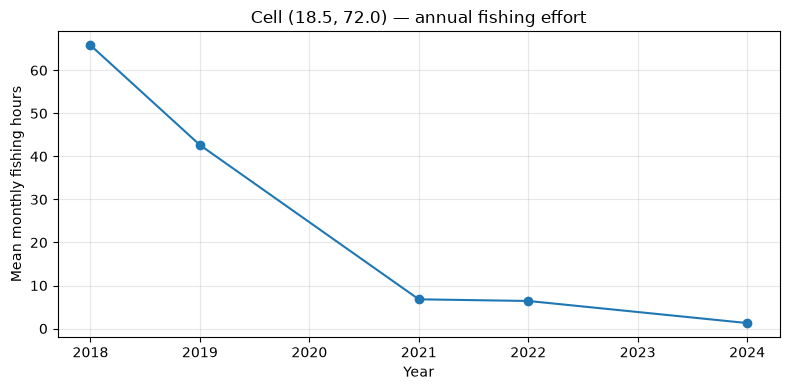
\includegraphics[width=\linewidth,height=0.20\textheight,keepaspectratio]
    {figures/cell_18_5_72_0.png}
    \textbf{(a)} Cell (18.5, 72.0)
\end{minipage}
\hfill
\begin{minipage}{0.48\textwidth}
    \centering
    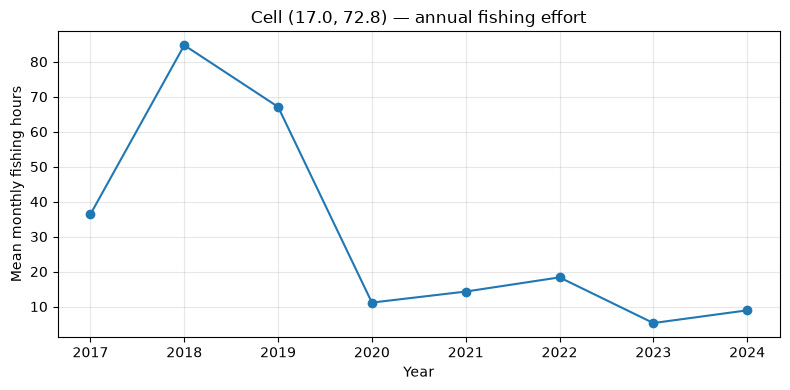
\includegraphics[width=\linewidth,height=0.20\textheight,keepaspectratio]
    {figures/cell_17_0_72_8.png}
    \textbf{(b)} Cell (17.0, 72.8)
\end{minipage}

\medskip

\begin{minipage}{0.48\textwidth}
    \centering
    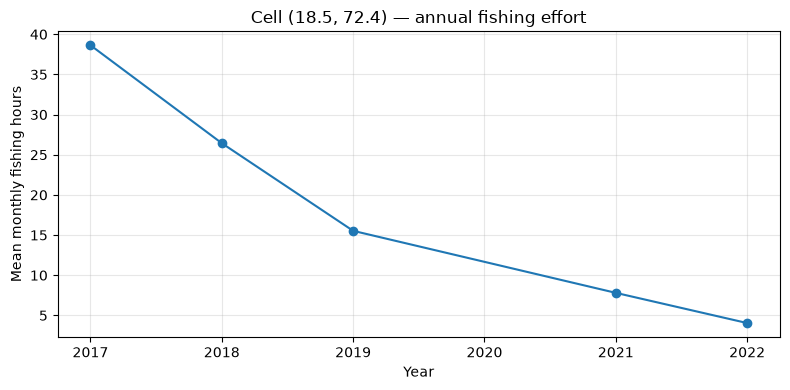
\includegraphics[width=\linewidth,height=0.20\textheight,keepaspectratio]
    {figures/cell_18_5_72_4.png}
    \textbf{(c)} Cell (18.5, 72.4)
\end{minipage}
\hfill
\begin{minipage}{0.48\textwidth}
    \centering
    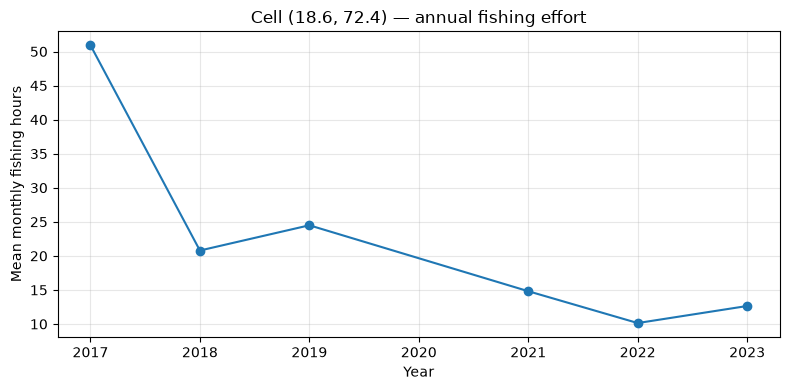
\includegraphics[width=\linewidth,height=0.20\textheight,keepaspectratio]
    {figures/cell_18_6_72_4.png}
    \textbf{(d)} Cell (18.6, 72.4)
\end{minipage}

\medskip

\begin{minipage}{0.48\textwidth}
    \centering
    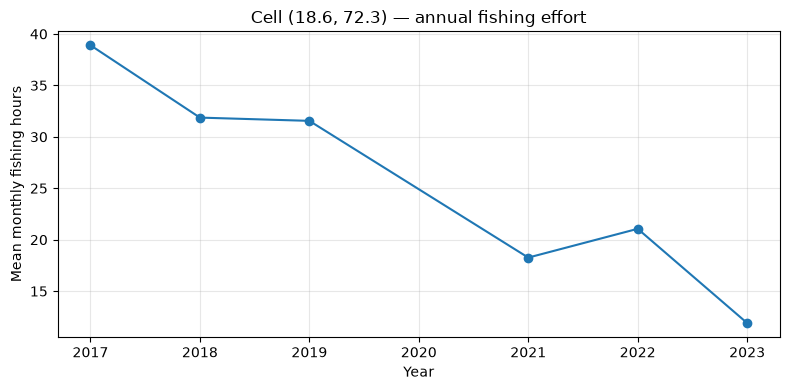
\includegraphics[width=\linewidth,height=0.20\textheight,keepaspectratio]
    {figures/cell_18_6_72_3.png}
    \textbf{(e)} Cell (18.6, 72.3)
\end{minipage}
\hfill
\begin{minipage}{0.48\textwidth}
    \centering
    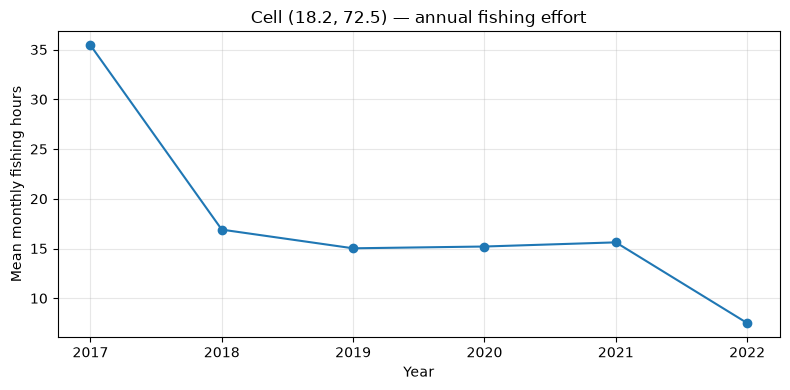
\includegraphics[width=\linewidth,height=0.20\textheight,keepaspectratio]
    {figures/cell_18_2_72_5.png}
    \textbf{(f)} Cell (18.2, 72.5)
\end{minipage}

\caption{Temporal variation in mean monthly fishing
effort across six geographical cells exhibiting
statistically significant declining trends.}
\label{fig:declining-cell-trends}
\end{figure}

\FloatBarrier


% ------------------------------------------------------------
% 4.3.3 Regions Exhibiting Increasing Fishing Effort
% ------------------------------------------------------------

\subsubsection{Regions Exhibiting Increasing Fishing Effort}

In contrast to the declining cells, 39 spatial
cells exhibited statistically significant
increasing fishing-effort trends.

Several of the strongest positive trends were
identified between approximately
$13.6^\circ$--$16.4^\circ$ N latitude and
$72.1^\circ$--$73.6^\circ$ E longitude.

The highest estimated positive slope was
observed at the cell located at
$13.6^\circ$ N and $73.6^\circ$ E, with
an estimated increase of 63.5021 mean
monthly fishing hours per year. The
corresponding $R^2$ value was 0.8170,
with a regression $p$-value of 0.0353.

These findings indicate that increasing and
declining fishing-effort trends were not
uniformly distributed across the study area.

\FloatBarrier



% Example figure:
% \begin{figure}[t]
%     \centering
%     \includegraphics[width=0.9\textwidth]{figures/example.png}
%     \caption{Example figure caption.}
%     \label{fig:example}
% \end{figure}

% Example table:
% \begin{table}[t]
% \centering
% \caption{Example table caption.}
% \label{tab:example}
% \begin{tabular}{lll}
% \toprule
% Column 1 & Column 2 & Column 3 \\
% \midrule
% Value & Value & Value \\
% \bottomrule
% \end{tabular}
% \end{table}

\section{Discussion}\label{sec:discussion}

\subsection{Summary and Interpretation of Main Findings}\label{subsec:disc-findings}

This study examined the spatiotemporal distribution and cell-level temporal trends of AIS-observed fishing effort using Global Fishing Watch (GFW) daily observations spanning 2012--2024, with trend analysis focused on 2015--2024 across 730,488 cleaned records, 1,930 unique vessels, and 23,846 spatial grid cells. Three patterns emerge from the analysis.

First, aggregate annual fishing effort increased markedly over 2015--2024, from 7,834.25~hours in 2015 to a peak of 991,262.66~hours in 2023, before declining to 846,165.09~hours in 2024; a temporary contraction in 2020 left 41,358.30~hours (Table~\ref{tab:annual-effort}). This trajectory closely tracks a major expansion in spatial coverage, from 578 observed cells in 2015 to 15,914 in 2024, with a simultaneous dip to 1,494 cells in 2020. Raw annual totals therefore cannot be interpreted as direct evidence of a uniform rise in fishing intensity. They reflect expanding AIS observability together with actual vessel activity, which is why cell-level trends are estimated from the coverage-normalized mean monthly fishing effort ($\overline{E}_{c,y}$; Eq.~\ref{eq:mean-monthly-effort}).

Second, accumulated fishing effort was concentrated in space rather than evenly distributed across the $-29.2^\circ$ to $40.0^\circ$ latitude and $32.0^\circ$ to $161.9^\circ$ longitude domain. The five highest-effort grid cells were located within $12.6^\circ$--$12.9^\circ$~N and $74.5^\circ$--$74.7^\circ$~E, led by cell $(12.8^\circ\text{ N}, 74.6^\circ\text{ E})$ with 22,251.96~fishing hours and 643 unique vessels (Table~\ref{tab:top-effort-cells}). Vessel counts across the five cells remained between 538 and 643, indicating sustained multi-vessel concentration in localized coastal fishing grounds.

Third, once temporal coverage was normalized and restricted to cells meeting the five-year eligibility threshold (at least three observed months per year), most eligible locations showed no significant linear change. Of the 8,697 examined cells, 8,140 (93.60\%) had insufficient data for trend estimation, leaving 557 eligible cells (Table~\ref{tab:trend-classification}). Among these, 511 (91.74\%) were classified as stable or statistically non-significant ($p \ge 0.05$). Significant directional trends were spatially localized. Thirty-nine cells (7.00\%) increased, with several of the strongest positive slopes between $13.6^\circ$--$16.4^\circ$~N and $72.1^\circ$--$73.6^\circ$~E, peaking at 63.5021 mean monthly fishing hours per year at $(13.6^\circ\text{ N}, 73.6^\circ\text{ E})$ ($R^2 = 0.8170$, $p = 0.0353$). Seven cells (1.26\%) declined, clustered further north between $17.0^\circ$--$18.6^\circ$~N and $72.0^\circ$--$72.8^\circ$~E, with slopes from $-10.8746$ to $-3.8394$ mean monthly fishing hours per year ($R^2 = 0.5152$--$0.9339$; Table~\ref{tab:declining-cells}, Fig.~\ref{fig:declining-cell-trends}). Local increases and declines therefore coexist with broad cell-level stability.

\subsection{Comparison with Previous Studies}\label{subsec:disc-comparison}

Our results both support and extend prior global and Indian Ocean AIS fisheries research. At the global scale, Kroodsma et~al.~\cite{kroodsma2018} established AIS-based apparent fishing effort as a viable framework for mapping industrial fishing footprints across 2012--2016. Using the updated GFW v3.0 dataset~\cite{gfw2025}, we extend observation coverage through December 2024 and move from global descriptive mapping to coverage-normalized, cell-level linear trend classification at native grid resolution.

At the regional scale, our coverage diagnostics are consistent with the FAO Global Atlas assessments for the Indian Ocean~\cite{taconet2019,murua2019,iotc2019}. Murua et~al.~\cite{murua2019} documented that AIS adoption in the Western Indian Ocean (FAO Area~51) relied heavily on lower-power Class~B transponders with uneven reception in the northern basin. IOTC~\cite{iotc2019} reported very poor AIS reception across much of the Eastern Indian Ocean (FAO Area~57), including the Bay of Bengal. These baseline reception constraints explain three features of our dataset: sparse early monthly observations in 2012--2014, the failure of 93.60\% of examined cells to meet the five-year trend filter, and the concentration of the highest-effort cells and significant trend clusters along the eastern Arabian Sea ($72.0^\circ$--$74.7^\circ$~E) despite a much wider spatial bounding box.

Methodologically, our workflow addresses concerns raised by European and basin-scale tracking studies. Natale et~al.~\cite{natale2015} emphasized that AIS reception gaps should not be treated as zero fishing activity; our pipeline therefore avoided zero-imputation for missing months and normalized annual totals by observed active months ($M_{c,y}$). Russo et~al.~\cite{russo2016} showed that AIS alone can underestimate fishing footprints relative to Vessel Monitoring Systems (VMS) and omits smaller vessels below statutory carriage thresholds. This constraint is particularly relevant in the Indian Ocean, where small-scale and artisanal fleets largely operate without AIS~\cite{murua2019}. Guiet et~al.~\cite{guiet2019} reported strong seasonal variability in Indian Ocean fishing effort, so differences in which months are observed across years ($M_{c,y} \ge 3$) may contribute to interannual variance in cell-level means. Utama et~al.~\cite{utama2021} showed, using Indonesian VMS records, that regulatory changes can drive spatial relocation of fishing effort in the Indian Ocean, and Welch et~al.~\cite{welch2022} found that intentional offshore AIS disabling obscures substantial vessel activity. Both studies caution that localized declines such as those at $17.0^\circ$--$18.6^\circ$~N may reflect fleet redistribution or changes in AIS transmission behavior rather than reduced fishing pressure alone.

\subsection{Limitations and Implications}\label{subsec:disc-limitations}

Several limitations inherent to the dataset and analytical design should be considered when interpreting these findings. First, AIS data capture only vessels equipped with active transponders, which excludes non-AIS artisanal and small-scale coastal fleets; progressive changes in transponder adoption or satellite reception over 2015--2024 can also influence observed effort trajectories~\cite{taconet2019,murua2019,russo2016,gfw2025}. Second, the analysis relies on pre-filtered \textit{fishing\_hours} without disaggregation by gear type, flag state, catch, or environmental covariates, so observed effort changes cannot be attributed to specific biological, economic, or regulatory drivers~\cite{natale2015,guiet2019,taconet2019}. Third, restricting trend estimation to cells with at least five valid annual observations excluded 93.60\% of examined cells and limited inference to persistently monitored grounds; within the 557 eligible cells, linear regression over 5--8~year series (Table~\ref{tab:declining-cells}) detects only monotonic linear change and does not capture non-linear dynamics. Fourth, quality checks identified 78 duplicate rows in the integrated dataset, which makes explicit deduplication necessary in reproducible AIS pipelines.

Despite these constraints, the study has clear implications for AIS-based fisheries monitoring. Analytically, raw multi-year fishing-hour totals should be evaluated alongside observed spatial cell counts and coverage-normalized metrics ($\overline{E}_{c,y}$), so that expanding surveillance coverage is not mistaken for uniform fishing intensification. Practically, pairing accumulated effort hotspots (Table~\ref{tab:top-effort-cells}) with spatially resolved trend classifications (Tables~\ref{tab:trend-classification}--\ref{tab:declining-cells}) identifies priority coastal corridors: the high-effort zone at $12.6^\circ$--$12.9^\circ$~N, the increasing zone at $13.6^\circ$--$16.4^\circ$~N, and the declining zone at $17.0^\circ$--$18.6^\circ$~N. In these corridors, integrating open-access AIS screening with national VMS records, fleet registries, and landings data can distinguish genuine shifts in fishing pressure from changes in vessel observability~\cite{natale2015,russo2016,utama2021,welch2022}.

\section{Conclusion}\label{sec:conclusion}

Summarize the main findings and contributions. Mention important limitations and possible directions for future work where appropriate.

% ------------------------------------------------------------
% Back matter
% ------------------------------------------------------------

\backmatter

\bmhead{Acknowledgements}

% Add acknowledgements here, or remove this section if not applicable.

\section*{Declarations}

\subsection*{Funding}
Not applicable.

\subsection*{Conflict of interest}
The authors declare no conflict of interest.

\subsection*{Ethics approval and consent to participate}
Not applicable.

\subsection*{Consent for publication}
Not applicable.

\subsection*{Data availability}
Not applicable.

\subsection*{Materials availability}
Not applicable.

\subsection*{Code availability}
Not applicable.

\subsection*{Author contribution}
Not applicable.

% ------------------------------------------------------------
% Optional appendix
% ------------------------------------------------------------

% \begin{appendices}
% \section{Additional Results}\label{sec:appendix-results}
% Add supplementary material here.
% \end{appendices}

% ------------------------------------------------------------
% References
% ------------------------------------------------------------

\bibliography{sn-bibliography}

\end{document}